\section{初等函数}

\begin{frame}{背景}
1
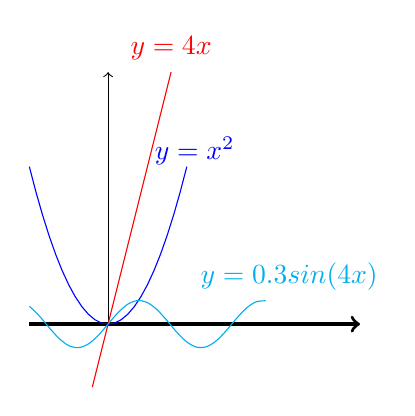
\begin{tikzpicture}
%画x和y轴坐标
\draw[very thick, ->](-1,0)--(3.2,0);
\draw[->](0,0)--(0,3.2);
\draw[red,domain=-0.2:0.8] plot(\x,4*\x) node at (0.8,3.5){$y=4x$};
\draw[blue,domain=-1:1] plot(\x,2*\x*\x) node at (1.1,2.2){$y=x^2$};
\draw[cyan,domain=-1:2,smooth] plot(\x,{0.3*sin(4*\x r)}) node at (2.3,0.6){$y=0.3sin(4x)$};
\end{tikzpicture}
\end{frame}
